\documentclass{article}
\usepackage{graphicx}
\usepackage{polski}
\usepackage[utf8]{inputenc}
\usepackage{amsfonts}
\usepackage{listings}
\usepackage{amssymb}
\usepackage{amsmath}
\usepackage{breqn}
\usepackage{blindtext}
\usepackage{titlesec}

\author{Piotr Koproń \and Bartłomiej Słupik}
\date{2023.03.03}
\title{Podejmowanie decyzji - projekt zaliczeniowy; wersja 0.1.0}

\begin{document}

\maketitle
\tableofcontents
\newpage

\section{Wstęp}
W niniejszym dokumencie przedstawione są założenia i projekt aplikacji zaliczeniowej z przedmiotu "Podejmowanie Decyzji".
System powinien umożliwiać użytkownikowi tworzenie rankingów obiektów, których pary mogą porównywać klienci.
Następnie wyliczany będzie ranking końcowy w oparciu o jedną z metod EVM i GMM.
W części 'Specyfikacja' przedstawione są dokładne założenia działania aplikacji z punktu widzenia użytkownika, takie jak
przypadki użycia, przykładowy schemat interakcji, czy plan wdrażania kolejnych funkcjonalności.
Następnie w części 'Projekt' zamieszczono plan od strony technicznek, w tym schemat działania back-endu i konstrukcję bazy danych.

\section{Specyfikacja}
\subsection{Zakres projektu}
\subsubsection{Cele projektu}
Podstawowym celem projektu jest przygotowanie aplikacji do grupowego podejmowania decyzji metodą AHP (metodą porównywania parami). \\
\begin{itemize}
    \item aplikacja powinna wykorzystywać metodę EVM i/lub GMM do tworzenia rankingów oraz odpowiednie metody 
    AIJ i/lub AIR do grupowania osądów (macierzy porównywania parami) pochodzących od różnych ekspertów. 
    \item aplikacja powinna - pozwalać na używanie tzw. skali fundamentalnej ale również na definiowanie
    swojej własnej skali porównań przez użytkownika, w tym bezpośrednio skali numerycznej. 
    \item aplikacja powinna działać w architekturze klient-serwer 
    \item aplikacja powinna umożliwiać pełny eksport danych rankingowych (wszystkich danych wejściowych) 
    do pliku JSON (przykładowy plik załączony w sekcji Ramowy Opis Projektu).
\end{itemize}

\subsubsection{Przykładowy Use Case, który powinien być możliwy do zrealizowania}
\begin{itemize}
    \item Facylitator
    \begin{itemize}
        \item Tworzy nowy ranking
        \begin{itemize}
            \item Definiuje nowe alternatywy
            \item Definiuje kryteria
            \item Definiuje pod-kryteria (jeśli to konieczne)
            \item Definiuje uczestników rankingu
            \item Określa parametry rankingu takie jak:
            \begin{itemize}
                \item Sposób liczenia rankingu (EVM / GMM etc).
                \item Czy ranking ma być kompletny czy nie kompletny
                \item Skale pomiarową
                \item Sposób liczenia niespójności rankingu
                \item Kolejność zadawanych pytań (losowa / konkretna)
                \item Datę i czas od której ranking ma być dostępny
                \item Datę i czas do której ranking ma być dostępny
            \end{itemize}
            \item Rozsyła zaproszenie do udziału w rankingu ekspertom (uczestnikom rankingu)
        \end{itemize}
    \end{itemize}

    \item Eksperci
    \begin{itemize}
        \item Odpowiadają na pytania o porównanie parami alternatyw (na jednym ekranie powinno znaleźć się jedno pytanie (jedno porównanie parami dwóch alternatyw)
        \item Odpowiadają na pytania o porównanie parami kryteriów (podobnie na jednym ekranie jedno porównanie)
        \item "Naciskają" guzik [submit], informujący system, że z ich strony ocena się zakończyła.
    \end{itemize}

    \item Facylitator
    \begin{itemize}
        \item Sprawdza zebrane wyniki
        \item Nadzoruje wykonanie rankingu
        \item Rozsyła wyniki uczestnikom/ekspertom procesu (oraz decydentom zewnętrznym).
        \item Eksportuje wszystkie dane procesu do formatu JSON. 
    \end{itemize}
\end{itemize}

\subsection{Architektura}
\begin{itemize}
	\item Serwer: REST-based ASP .NET Core (C\#)
	\item Klient: React+Next.js+TypeScript - zgodnie z mockami w osobnych dokumentach
	\item Wewnętrzne REST API - zgodnie z osobnym dokumentem
	\item Baza danych - EntityFramework Code First
\end{itemize}

\subsection{Konfguracja}
\begin{itemize}
	\item Frontend developement
	\begin{itemize}
        \item cd reporoot/web
        \item npm run dev
        \item Aplikacja uruchomiona na http:\\localhost:3000
	\end{itemize}
	\item Backend
\end{itemize}
	
\subsection{Zarządzanie testowaniem}
BLOCKED BY: Brak zatwierdzenia specyfikacji przez Klienta 

\subsection{Zarządzanie ryzykiem}
Podstawowym źródłem ryzyka są nieprzewidziane okoliczności. Zalecane ostrożne estymaty czasu pracy nad funkcjonalnościami.
Przy tworzeniu aplikacji będą priorytetyzowane funkcjonalności krytyczne ponad błędami oraz aspektami wizualnymi i płynnścią działania.


\pagebreak
\section{Część projektowa}
\subsection{Założenia przed rozpoczęciem realizacji}
\begin{itemize}
    \item Wykonanie testowej bazy w technice Code First aby opanować sprawne tworzenie migracji w Entity Framework
\end{itemize}

\subsection{Ograniczenia}
\begin{itemize}
    \item Użytkownik będzie korzystał z aplikacji poprzez przeglądarkę internetową. Nie przewidujemy wykonania aplikacji mobilnej.
\end{itemize}

\subsection{Wzorce architektoniczne}
\begin{itemize}
    \item Aplikacja będzie działać w modelu klient-serwer, opierając się na komunikacji przy pomocy kontrolera i modelu (MVC)
    \item Serwer będzie podzielony na warstwy przejmujące różne jego role, tj. dostępu aplikacji, obliczeniowa, 
    dostępu do bazy danych.
\end{itemize}

\pagebreak
\subsection{Diagram komponentów}
\begin{figure}[h!]
    \centering
    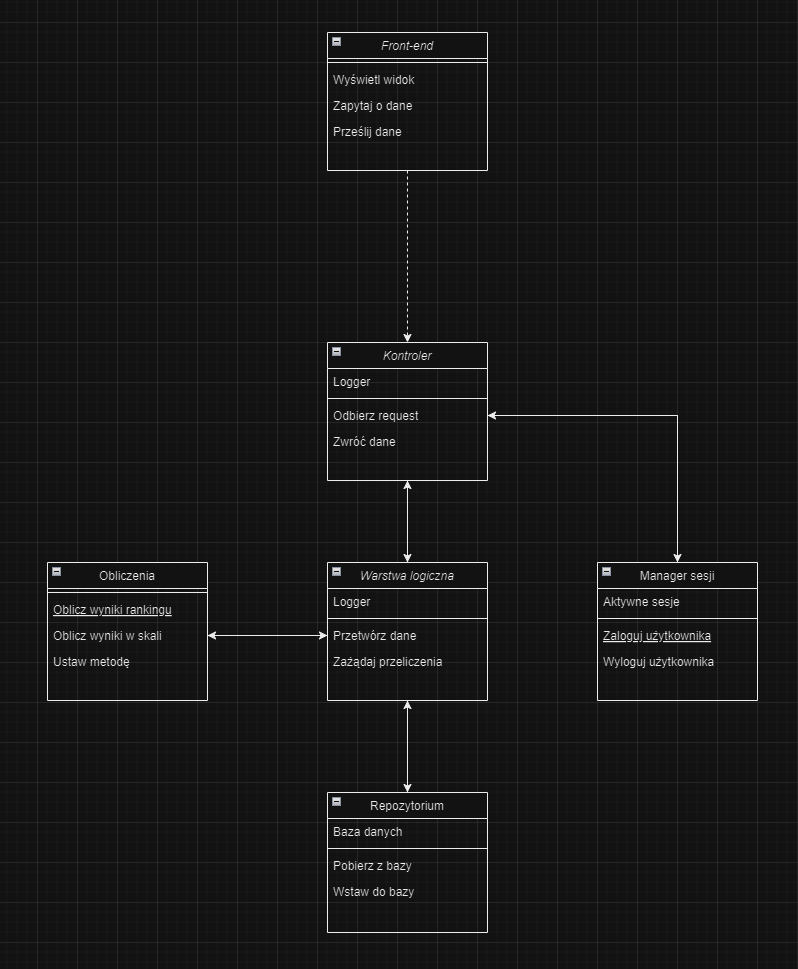
\includegraphics[width=\linewidth]{component-diagram.PNG}
    \caption{Diagram komponentów. Naszkicowane moduły odpowiadają w dużej mierze docelowym klasom, które będą wykonywały te zadania.}
\end{figure}

\pagebreak
\subsection{Diagram przepływu danych}
\begin{figure}[h!]
    \centering
    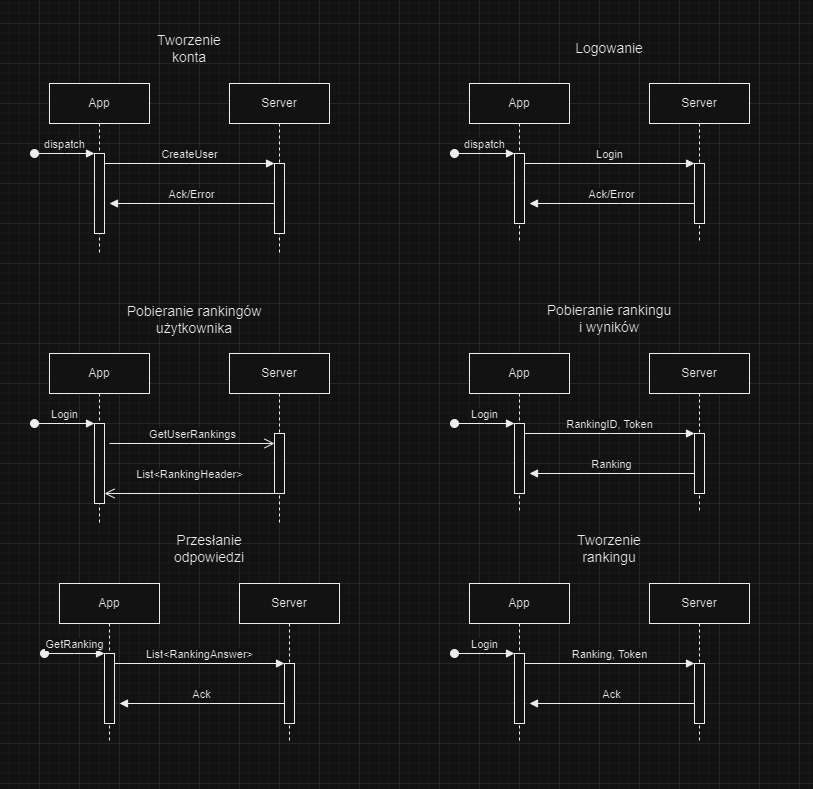
\includegraphics[width=\linewidth]{data-flow-diagram.PNG}
    \caption{Diagram przepływu danych. Opisane sekwencje są odzwierciedlane przez projektowane API.}
\end{figure}

\pagebreak
\subsection{Model bazy danych}
\begin{figure}[h!]
    \centering
    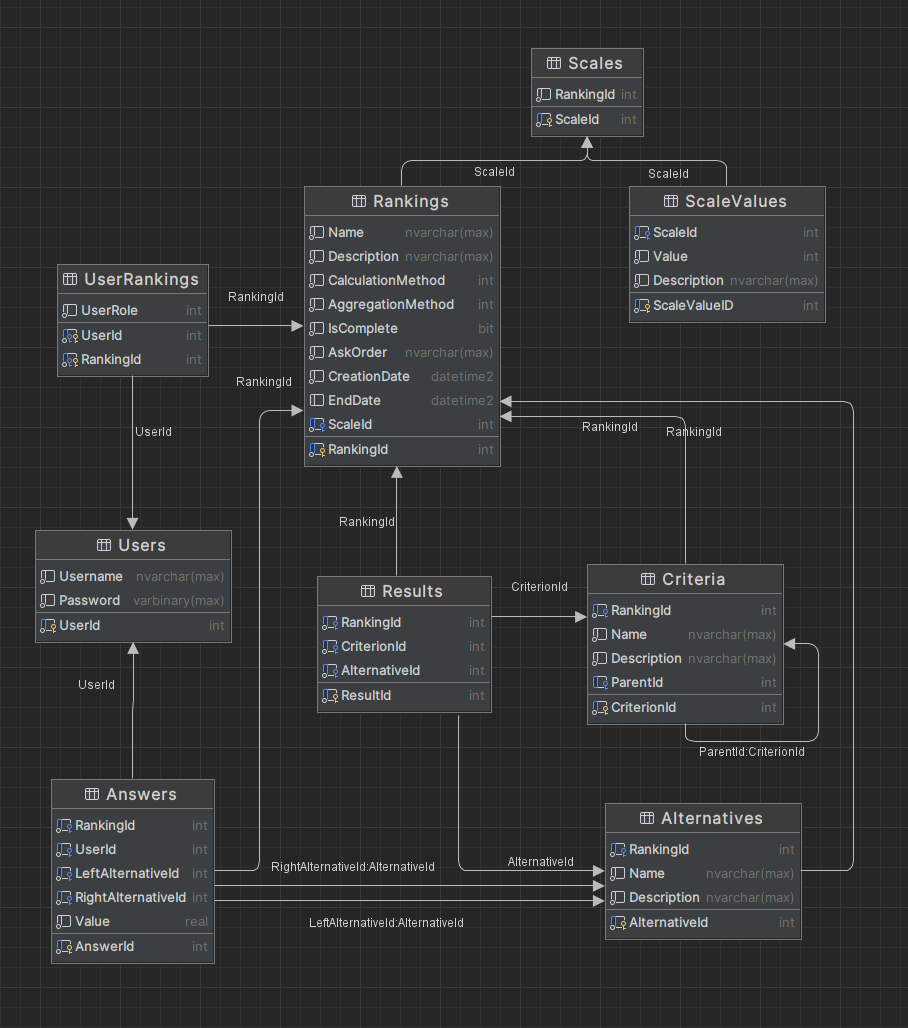
\includegraphics[width=\linewidth]{db-diagram-vert.PNG}
    \caption{Schemat bazy danych}
\end{figure}

\pagebreak
\subsection{Harmonogram realizacji}
\begin{itemize}
    \item Implementacja modelu i kontrolera zwracającego mockowe dane (21.11.2023)
    \item Stworzenie warstwy dostępu do bazy danych i funkcjonalności tworzenia i usuwania obiektów (5.12.2023)
    \item Zaimplementowanie algorytmów obliczających rankingi wraz z testami (19.12.2023)
    \item Ulepszenie komponentu logowania użytkownika o lepsze bezpieczeństwo i zachowanie sesji (2.01.2024)
\end{itemize}

\end{document}